\documentclass[10pt]{beamer}\usepackage[]{graphicx}\usepackage[]{color}
% maxwidth is the original width if it is less than linewidth
% otherwise use linewidth (to make sure the graphics do not exceed the margin)
\makeatletter
\def\maxwidth{ %
  \ifdim\Gin@nat@width>\linewidth
    \linewidth
  \else
    \Gin@nat@width
  \fi
}
\makeatother

\definecolor{fgcolor}{rgb}{0.345, 0.345, 0.345}
\newcommand{\hlnum}[1]{\textcolor[rgb]{0.686,0.059,0.569}{#1}}%
\newcommand{\hlstr}[1]{\textcolor[rgb]{0.192,0.494,0.8}{#1}}%
\newcommand{\hlcom}[1]{\textcolor[rgb]{0.678,0.584,0.686}{\textit{#1}}}%
\newcommand{\hlopt}[1]{\textcolor[rgb]{0,0,0}{#1}}%
\newcommand{\hlstd}[1]{\textcolor[rgb]{0.345,0.345,0.345}{#1}}%
\newcommand{\hlkwa}[1]{\textcolor[rgb]{0.161,0.373,0.58}{\textbf{#1}}}%
\newcommand{\hlkwb}[1]{\textcolor[rgb]{0.69,0.353,0.396}{#1}}%
\newcommand{\hlkwc}[1]{\textcolor[rgb]{0.333,0.667,0.333}{#1}}%
\newcommand{\hlkwd}[1]{\textcolor[rgb]{0.737,0.353,0.396}{\textbf{#1}}}%
\let\hlipl\hlkwb

\usepackage{framed}
\makeatletter
\newenvironment{kframe}{%
 \def\at@end@of@kframe{}%
 \ifinner\ifhmode%
  \def\at@end@of@kframe{\end{minipage}}%
  \begin{minipage}{\columnwidth}%
 \fi\fi%
 \def\FrameCommand##1{\hskip\@totalleftmargin \hskip-\fboxsep
 \colorbox{shadecolor}{##1}\hskip-\fboxsep
     % There is no \\@totalrightmargin, so:
     \hskip-\linewidth \hskip-\@totalleftmargin \hskip\columnwidth}%
 \MakeFramed {\advance\hsize-\width
   \@totalleftmargin\z@ \linewidth\hsize
   \@setminipage}}%
 {\par\unskip\endMakeFramed%
 \at@end@of@kframe}
\makeatother

\definecolor{shadecolor}{rgb}{.97, .97, .97}
\definecolor{messagecolor}{rgb}{0, 0, 0}
\definecolor{warningcolor}{rgb}{1, 0, 1}
\definecolor{errorcolor}{rgb}{1, 0, 0}
\newenvironment{knitrout}{}{} % an empty environment to be redefined in TeX

\usepackage{alltt}

\beamertemplatenavigationsymbolsempty

\usepackage{booktabs}
\usepackage{colortbl}

\usepackage{tikz}
\usetikzlibrary{positioning,shapes.misc,calc,backgrounds,scopes} 
\tikzset{boxed/.style={
  thick,
  draw=black,
  top color=white,
  text height=1.5ex,
  text depth=.25ex
}}


\newcommand\lo{\ensuremath{\boldsymbol{-}}}
\newcommand\hi{\ensuremath{\boldsymbol{+}}}

\title{Response Surface Methodology}
\author{BIOE 498/598 PJ}
\date{Spring 2021}
\IfFileExists{upquote.sty}{\usepackage{upquote}}{}
\begin{document}
\frame{\titlepage}


\begin{frame}{Last time: The method of steepest ascent}

\begin{columns}
\begin{column}{0.6\textwidth}
  \begin{itemize}
    \item Begin with a FF+CP design.
    \item<2-> Follow path of steepest ascent until the model breaks.
    \item<3-> New FF+CP; repeat steepest ascent.
    \item<4-> Stop when model detects lack of fit.
    \item<5-> \textbf{Today}: Fitting a model to a curved response surface.
  \end{itemize}
\end{column}
\begin{column}{0.4\textwidth}
  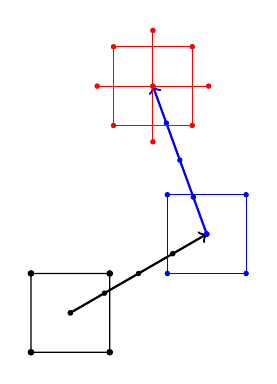
\begin{tikzpicture}
    \begin{scope}[scale=0.5]
      \filldraw [black] (1,1) circle (2pt) -- (-1,1) circle (2pt) -- (-1,-1) circle (2pt) -- (1,-1) circle (2pt) -- (1,1);
      \fill [black] (0,0) circle (2pt);
      \onslide<2->{
        \draw [thick,black,rotate=30,->] (0,0) -- (4,0) coordinate (c2);
        \fill [black,rotate=30] (0,0) circle (2pt) ++ (1,0) circle (2pt) ++ (1,0) circle (2pt) ++ (1,0) circle (2pt) ++ (1,0) circle (2pt);
      }
      \onslide<3->{
        \fill [blue] (c2) circle (2pt) +(1,1) circle (2pt) +(-1,1) circle (2pt) +(-1,-1) circle (2pt) +(1,-1) circle (2pt);
        \draw [blue] ($(c2) +(1,1)$) -- ++(-2,0) -- ++(0,-2) -- ++(2,0) -- cycle;
        \draw [thick,blue,rotate=110,->] (c2) -- ++(4,0) coordinate (c3);
        \fill [blue,rotate=110] (c2) circle (2pt) ++ (1,0) circle (2pt) ++ (1,0) circle (2pt) ++ (1,0) circle (2pt) ++ (1,0) circle (2pt);
      }
      \onslide<4->{
        \fill [red] (c3) circle (2pt) +(1,1) circle (2pt) +(-1,1) circle (2pt) +(-1,-1) circle (2pt) +(1,-1) circle (2pt);
        \draw [red] ($(c3) +(1,1)$) -- ++(-2,0) -- ++(0,-2) -- ++(2,0) -- cycle;
      }
      \onslide<5->{
        \fill [red] (c3) +(1.414,0) circle (2pt) +(0,1.414) circle (2pt) +(-1.414,0) circle (2pt) +(0,-1.414) circle (2pt);
        \draw [red] (c3) -- +(1.414,0) (c3) -- +(-1.414,0) (c3) -- +(0,1.414) (c3) -- +(0,-1.414);
      }
    \end{scope}
  \end{tikzpicture}
\end{column}
\end{columns}

\end{frame}

\begin{frame}{Fitting models with curvature}

\begin{itemize}
  \item We need two things to model a curved response surface:
    \begin{enumerate}
      \item A model that is flexible enough to curve.
      \item Data that can detect the curvature.
    \end{enumerate}
  \item<2-> The optimal operating conditions correspond to a maximum in the response surface.
  \item<2-> We need models that can model maxima.
  \item<3-> FO + TWI models are curved, but are rarely bounded.
\end{itemize}

\onslide<4->{
  \[ y = 20 + 3.6x_1 - 1.8x_2 - 0.6x_1x_2 \]
  \medskip
  Set $x_2=0$, then $y\rightarrow\infty$ as $x_1\rightarrow\infty$.
}

\end{frame}

\end{document}
